%% LyX 2.0.8.1 created this file.  For more info, see http://www.lyx.org/.
%% Do not edit unless you really know what you are doing.
\documentclass[english]{article}
\usepackage[T1]{fontenc}
\usepackage[latin9]{inputenc}
\usepackage{graphicx}
\usepackage{babel}
\begin{document}

\title{Can You Win This Hot New Game Show?}


\author{Dan Schlauch}


\date{March 6, 2016}

\maketitle
From the FiveThirtyEight Riddler

http://fivethirtyeight.com/features/can-you-win-this-hot-new-game-show/

\emph{Two players go on a hot new game show called \textquotedblleft{}Higher
Number Wins.\textquotedblright{} The two go into separate booths,
and each presses a button, and a random number between zero and one
appears on a screen. (At this point, neither knows the other\textquoteright{}s
number, but they do know the numbers are chosen from a standard uniform
distribution.) They can choose to keep that first number, or to press
the button again to discard the first number and get a second random
number, which they must keep. Then, they come out of their booths
and see the final number for each player on the wall. The lavish grand
prize \textemdash{} a case full of gold bullion \textemdash{} is awarded
to the player who kept the higher number. Which number is the optimal
cutoff for players to discard their first number and choose another?
Put another way, within which range should they choose to keep the
first number, and within which range should they reject it and try
their luck with a second number?}


\part*{Solution}

We can think about this by dividing the probabilities into the four
possible ``first-press'' outcomes. These four come from Player A
accepts/represses and Player B accepts/represses.

If they both repress, it's easy... its essentially a coinflip. This
happens with probability $a\times b$

If both accept, it's now a competition between a $Uniform\left(a,1\right)$
and a $Uniform\left(b,1\right)$ random variable. This happens with
probability $\left(1-a\right)\left(1-b\right)$.

Similarly, when one accepts and the other represses, we have a competition
between a $Uniform\left(0,1\right)$ and a $Uniform\left(x,1\right)$.

We can write out the total probability as follows

\begin{eqnarray*}
P\left(Win_{A}|a,b\right) & = & P\left(Win_{A}|X_{1}<a,Y_{1}<b\right)+P\left(Win_{A}|X_{1}>a,Y_{1}>b\right)+\\
 &  & P\left(Win_{A}|X_{1}<a,Y_{1}>b\right)+P\left(Win_{A}|X_{1}>a,Y_{1}<b\right)\\
 & = & ab\left[\frac{1}{2}\right]+\left(1-a\right)\left(1-b\right)\left[.5\frac{\left(1-a\right)}{\left(1-b\right)}+\frac{\left(1-b\right)-\left(1-a\right)}{\left(1-b\right)}\right]+\\
 &  & b\left(1-a\right)\left[1-\frac{\left(1-a\right)}{2}\right]+a\left(1-b\right)\left[\frac{\left(1-b\right)}{2}\right]
\end{eqnarray*}


To find the optimal value for $a$ given $b$, we simply differentiate
and set equal to zero to get the max. 
\[
\frac{d}{da}P\left(Win_{A}|a,b\right)=b\left[\frac{1}{2}\right]+\left[b-a\right]+\left[-ab\right]+\left(1-b\right)\left[\frac{\left(1-b\right)}{2}\right]=0
\]


Player A and Player B are in mirror situations, so to find an unbeatable
strategy we need to find a value for $a$ (or $b$) such that they
are each other's maximum. So we do this by setting $a=b=x$

Setting $\frac{d}{da}P\left(Win_{A}|a,b\right)=0$ and finding the
equilibrium where $a=b$
\begin{eqnarray*}
x\left[\frac{1}{2}\right]+\left[x-x\right]+\left[-x^{2}\right]+\frac{x^{2}-2x+1}{2} & = & 0\\
-\frac{1}{2}x^{2}-\frac{1x}{2}+\frac{1}{2} & = & 0
\end{eqnarray*}
Using the quadratic formula we get
\begin{eqnarray*}
x & = & \sqrt{\frac{5}{4}}-\frac{1}{2}\\
x & = & 0.61803
\end{eqnarray*}
In other words, using a cutoff of $\approx.61803$ is an unbeatable
strategy. But it may not be the best if your opponent is less than
optimal.

\begin{figure}


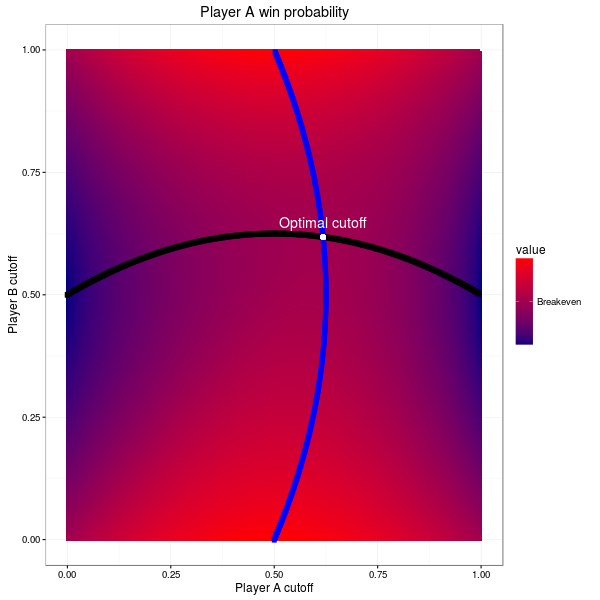
\includegraphics{gameshow_heatmap}\caption{Player A Win Probability: Black highlights optimal play for Player
B given Player A's cutoff. The white dot is the unbeatable cutoff
for both players.}


\end{figure}

\end{document}
